\part{Distance control}

\chapter{Modelling}
In this part, we'll focus on the modelling and the control of the distance between two satellites using the drag force as the control input of the system. First, we'll considerer that the orientation of the satellite is instantaneous and therefore, the drag force can be modified instantaneous. The Earth and the satellite is assumed to be a point mass to simplify the system. \\
The Satellite is mainly subjected to three forces: the gravity, the drag force and the sun radiation. Thus, the second law of Newton gives:
\[
\sum \vec{F} = m_{sat} \vec{a} = \vec{F_g} + \vec{F_D} + \vec{F_{rad}}
\]
with the gravity can be modeled by:
\[
\vec{F_g} = -G\frac{m_earth \cdot m_sat}{||\vec{p}||^3} \vec{p}
\]
where $\vec{p}$ is the vector position of the satellite (vector from the earth center to the mass center of the satellite in the inertital frame). The modelization of the $\vec{F_D}$ and $\vec{F_{rad}}$ are explained in the next section.
\section{Disturbance Models}
\subsection{Aerodynamic Drag Force}
The satellite is subjected to a aerodynamic drag force due to the atmosphere. The collisions with the air caused a force in the opposite direction of the velocity of the satellite. the force was modeled by Lord Rayleigh[ref]:
\[
\vec{F_D} = -\frac{1}{2} \rho \cdot C_D \cdot A_{\perp} ||\vec{v}|| \vec{v}
\]
where $\rho$ is the density of the air, $C_D$ is the drag coefficient, $A_{\perp}$ is the area that is perpendicular of the velocity of the satellite $\vec{v}$. \\
The drag coefficient $C_D$ and the perpendicular area $A_{\perp}$ depend of the orientation of the satellite. Therefore, this force can be used as a input for the control of the position and the velocity of the satellite. \\\
The density of the air depends of the altitude of the satellite, of the air temperature but we considered to be constant in our case to simplify the modelization. $\rho$ is chosen to be equal to $1.454 \cdot 10^-13$ $[\frac{Kg}{m^3}]$ based to the  empirical model of the Committee on Space Research (COSPAR) International Reference Atmosphere [Ref]. \\ %J. R. Wertz, Spacecraft Attitude Determination and Control. Kluwer Academic Publishers, 1st ed., 1994.
The drag coefficient as said before is orientation dependant. The maximum value of $C_D$ is equal to 1.05 for a non tilited cubed as shown on the figure \ref{drag_coef} and equal to 0.80 for an angled cubed. In our modelization, we will assume that the drag coefficient is constant and equal to 1(not sure which value take) in order to simplified the equation. \\
\begin{table}[H]
	\begin{minipage}[b]{0.49\linewidth}
		\centering
		\begin{figure}[H]
			\centering
			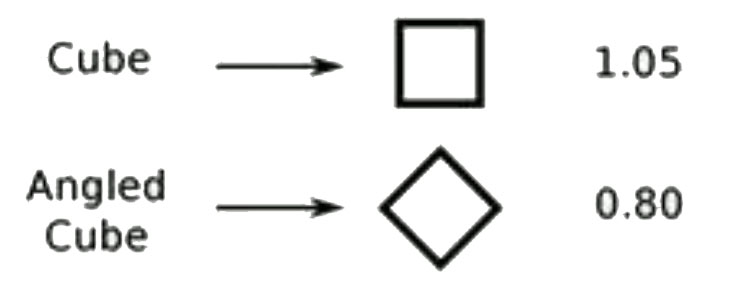
\includegraphics[width=0.8\linewidth]{figures/drag_coef}
			\caption{description needed}
			\label{fig:MW}
		\end{figure}
	\end{minipage}\hfill
	\begin{minipage}[b]{0.49\linewidth}
		\centering
		\begin{figure}[H]
			\centering
			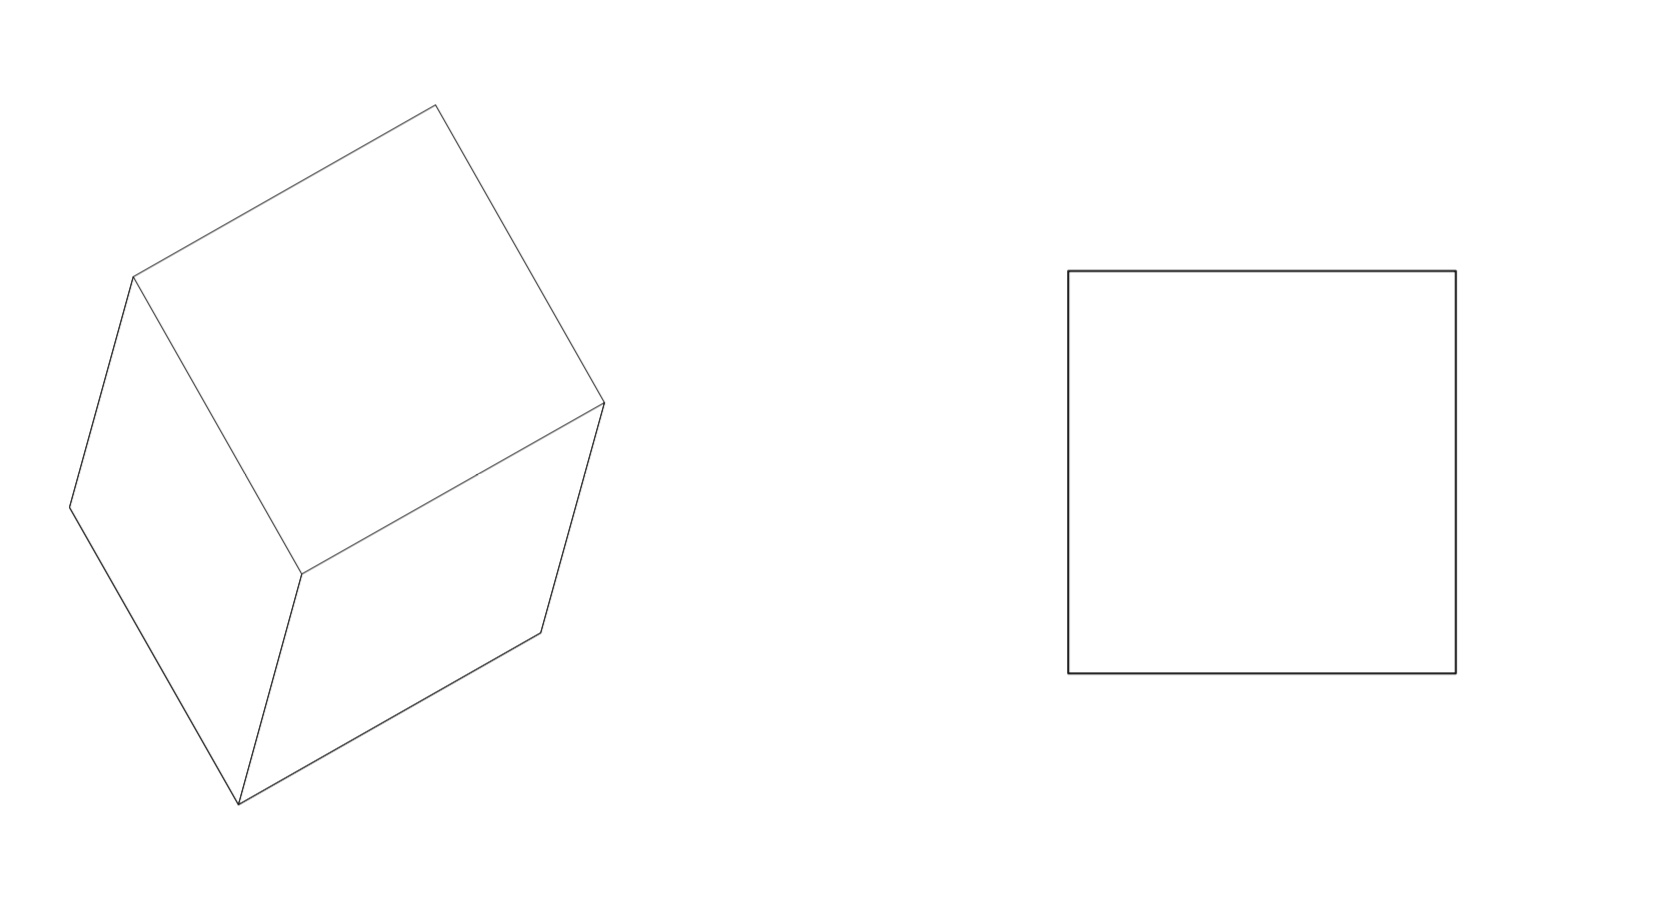
\includegraphics[width=1\linewidth]{figures/a_prep}
			\caption{description needed}
			\label{fig:cub}
		\end{figure}
	\end{minipage}
\end{table}
Therefore, the only parameter that we control is the perpendicular area $A_{\perp}$. The maximum and minimum value of $A_{\perp}$ are represented at the figure\ref{a_perp}. Thus, the minimum value is the surface of a square of 10cm of dimension ($A_{\perp} = 100cm^2$) and the maximum value is the surface of an hexagone of 10cm of dimension ($A_{\perp} = \frac{3\sqrt{3}}{2} 100cm^2$).
Thus, the drag force can be expressed as the following. 
\[
\vec{F_D} = -u ||\vec{v}|| \vec{v}
\]
with u is the control input and it can take value between $7.27 \cdot 10^{-16}$ and $1.888 \cdot 10^{-15}$.
\subsection{Solar radiation}
Due to low earth orbit flying, the surface of the CubeSat will absorb or reflect the solar radiation, nevertheless, these two situations will alter the CubeSat, which will produce a torque about the satellite center of mass(CoM). 

The torque around CoM is given by:
\begin{flalign}
	N_{rad} = F_{rad} \times R_{CoM}
	\label{eq:tor}
\end{flalign}
where $F_{rad}$  is the solar radiation  and $R_{CoM}$ is the vector from the centre of mass to the geometric centre of radiation

The solar radiation $F_{rad}$ can be expressed as:
\begin{flalign}
	F_{rad} = C_{a} P A
	\label{eq:Pres}
\end{flalign}
where $C_{a}$ is absorption constant of the radiated area and $P$ is the solar flux, while  $A$ is the radiated area
\section{State Space Representation}
The state of the system is the vector position and the vecteur velocity in the inertia frame:
\[
\vec{x} = \left[ \begin{array}{c} \vec{p} \\ \vec{v} \end{array} \right]
\]
The equation of (I don't remember the name of the equation xdot = f(x,u) + u) is given by:
\begin{flalign}
\dot{\vec{x}} &= \left[ \begin{array}{c} \dot{\vec{p}} \\ \dot{\vec{v}} \end{array} \right] = \left[ \begin{array}{c} \vec{v} \\ \vec{a} \end{array} \right] \\
 &= \left[ \begin{array}{c} \vec{v} \\ \frac{1}{m_{sat}}(-G\frac{m_{earth} \cdot m_{sat}}{||\vec{p}||^3} \vec{p}) - u ||\vec{v}|| \vec{v} + F_{rad} \end{array} \right] \\
 &= \vec{f(x)} + u \cdot \vec{g(x)} + \vec{\delta(x,t)}
\end{flalign}
with 
\[
\vec{f(x)} = \left[ \begin{array}{c} \vec{v} \\ -G\cdot m_{earth} \frac{\vec{p}}{||\vec{p}||^3} \end{array} \right], \ \vec{g(x)} = \left[ \begin{array}{c} \vec{0} \\ - \frac{1}{m_{sat}}||\vec{v}||\vec{v} \end{array} \right]
\]
and $\vec{\delta(x,t)}$ reprensent the influence all the disturbances.
\chapter{Distance control design}